\documentclass[11pt]{article}
\usepackage{amsmath} % Math
\usepackage{amssymb} % Math symbols
\usepackage[english]{babel} % Language
\usepackage{fancyhdr} % Header
\usepackage[a4paper, total={15cm, 20cm}]{geometry} % Dimensions of the paper and the text area
\usepackage[utf8]{inputenc} % encoding in UTF, needed for umlauts if German
\usepackage{mathtools} % Text above arrows
\usepackage{msc} % Drawing MSCs
\usepackage{multicol} % Multiple columns
\usepackage[explicit]{titlesec} % Automatic section titles
\usepackage{tikz} % Diagrams
\usetikzlibrary{arrows.meta, automata, shapes, matrix,positioning}
\usepackage{enumitem}   % Enumeration item
\usepackage{float}
\usepackage{verbatim}
\usepackage{subcaption} 


% Other packages that might be useful in the future
%\usepackage{lingmacros}
%\usepackage{tree-dvips}
%\usepackage{ulem}
%\usepackage{amsthm}
%\usepackage{amsbsy}
%\usepackage{textcomp,gensymb}
%\usepackage{graphicx}
%\usepackage{mathtools}

% Custom variant of msc environment:
% - No "msc" keyword, longer partial messages
% - Increased vertical distance between messages
% - Less distance to the frame left and right
% - Less distance between header and processes
% - Less distance between footer and frame
% - Passing all given options down to the msc environment
\newenvironment{cmsc}[1][]{\msc[msc keyword={}, self message width=1.1cm, level height=0.6cm, environment distance=1.2cm, head top distance=0.75cm, foot distance=0.5cm, #1]}{\endmsc}

% No indentation at new paragraphs
\setlength{\parindent}{0pt}

% Distance between columns
\setlength{\columnsep}{1cm}
% Vertical line between columns
\setlength{\columnseprule}{0.5pt}
\def\columnseprulecolor{\color{gray}}

% Settings
\newcommand{\sheetNr}{5}
\newcommand{\red}[1]{\color{red}#1\color{black}}

%% Header
\fancyhf{}
\pagestyle{fancy}
\lhead{Model Checking Exercise Sheet \sheetNr}
\rhead{Aaron Grabowy: 345766\\ Timo Bergerbusch: 344408\\ Felix Linhart: 318801}
\setlength{\headheight}{40pt}

%% Automatic section titles
\titleformat{\section}{\normalfont\Large\bfseries}{}{0em}{Exercise #1}
\titleformat{\subsection}{\normalfont\large\bfseries}{}{0em}{#1)}

\begin{document}
	
\section{1}
\subsection{a}
\begin{itemize}
	\item $\alpha_1 = a^*.(b.a^+)^\omega + a^*.(b.a^+)^*.b.a^\omega$
	\item $\alpha_2 = ((c.(b.c)^*.a+b).a)^\omega$
\end{itemize}

\subsection{b}

\begin{figure}[H]
\begin{subfigure}[c]{0.45\textwidth}
	$\mathcal{B}_1$:\\
\begin{tikzpicture}[shorten >=1pt,node distance=2cm,on grid,auto] 
%	\node[state, initial, initial text =] (s0) {$s_0$};
%	\node[state, above right = of s0] (s1) {$s_1$};
%	\node[state, right = of s1] (s2) {$s_2$};
%	\node[state, below right = of s0] (s3) {$s_3$};
%	\node[state, below = of s3] (s4) {$s_4$};
%	\node[state, right = of s4] (s5) {$s_5$};
%	
%	\path[->] 	(s0) edge[bend left = 20] node {$a$} (s1)
%	(s1) edge[bend left = 20] node {$b$} (s2)
%	(s2) edge[bend left = 20] node {$b$} (s1)
%	(s1) edge[bend left = 20] node {$b$} (s0)
%	(s0) edge[bend left = 0] node {$a$} (s3)
%	(s3) edge[bend left = 0] node {$c$} (s4)
%	(s4) edge[bend left = 20] node {$c$} (s5)
%	(s5) edge[bend left = 20] node {$c$} (s4)
%	(s4) edge[bend left = 20] node {$c$} (s0);
	\node[state, initial, initial text =] (s0) {$s_0$};
	
	\node[state, right = of s0,rectangle] (s1) {$s_1$};
	\node[state, above right = of s1] (s2) {$s_2$};
	\node[state, right = of s2] (s3) {$s_3$};
	
	\node[state, below right = of s1] (s4) {$s_4$};
	\node[state, below= of s4] (s5) {$s_5$};
	
	\path[->] 	(s0) edge[loop above] node {$b\lor c$} (s0)
	(s0) edge node {$a$} (s1)
	(s1) edge[bend left = 20] node {$b$} (s2)
	(s2) edge[bend left = 20] node {$a$} (s1)
	(s2) edge[bend left = 20] node {$b$} (s3)
	(s3) edge[bend left = 20] node {$b$} (s2)
	(s1) edge node {$c$} (s4)
	(s4) edge[bend left = 20] node {$c$} (s5)
	(s5) edge[bend left = 20] node {$c$} (s4)
	(s5) edge[bend left = 20] node {$a$} (s1);
\end{tikzpicture}
\end{subfigure}
\begin{subfigure}[c]{0.45\textwidth}
	$\mathcal{B}_2$:\\
\begin{tikzpicture}[shorten >=1pt,node distance=3cm,on grid,auto] 
	\node[state, initial, initial text =] (s0) {$s_0$};
	\node[state, above right = of s0, rectangle] (s1) {$s_1$};
%	\node[state, right = of s1] (s2) {$s_2$};
	\node[state, below right = of s0, rectangle] (s3) {$s_3$};
	\node[state, right = of s3] (s4) {$s_4$};
	\node[state, below = of s3] (s5) {$s_5$};
	
	\path[->] 	(s0) edge[loop above] node {true}	(s0)
	(s0) edge node {$c$} (s1)
	(s1) edge[loop above] node {$c$}	(s1)
%	(s1) edge node {$a \lor b$} (s2)
%	(s2) edge[loop above] node {true}	(s2)
	(s0) edge node {$a \lor b$} (s3)
%	(s3) edge[loop below] node {$a \lor b$}	(s3)
	(s3) edge[bend left = 20] node {$a$} (s4)
	(s4) edge[bend left = 20] node {$b$} (s3)
	(s3) edge[bend left = 20] node {$b$} (s5)
	(s5) edge[bend left = 20] node {$a$} (s3)
	(s4) edge[loop right] node {$a$} (s4)
	(s5) edge[loop right] node {$b$} (s5);
\end{tikzpicture}
\end{subfigure}
\end{figure}

\subsection{c}
\subsubsection*{$\mathcal{L}_\omega^1$:}
Since the stated NBA is already a DBA there obviously exists one.
\subsubsection*{$\mathcal{L}_\omega^2$:}

The proof follows the principle of the proof of $(A + B)^*.A^\omega$. In this case $A$ corresponds to $c$ and $B$ to $b$.

Assuming there exists a DBA $\mathcal{A}$ with $\mathcal{L_\omega(A) = L}_\omega^2 =: L$.

Note that $\mathcal{L}_\omega((c + b)^*.c^\omega) \subseteq L$, since $c$ occurs infinitely many times and $a$ and $b$ only occur finitely many times.

Following the proof yields a sequence $n_1, n_2, \ldots$ of natural numbers and a sequence $q_1, q_2, \ldots$ of accepting states such that $\delta(q_0, c^{n_1}bc^{n_2} \ldots c^{n_{i-1}}bc^{n_i}) = \{q_i\}$.

Since $Q$ is finite, there ex. $i < j$ such that $\delta(q_0, c^{n_1}b \ldots bc^{n_i}) = \delta(q_0, c^{n_1}b \ldots bc^{n_j})$.

Thus, $\mathcal{A}$ has an accepting run on $c^{n_1}b \ldots bc^{n_i} (bc^{n_{i+1}} \ldots bc^{n_j})^\omega \notin L$, since $c$ and $b$ occur infinitely many times.
This contradicts $\mathcal{L_\omega(A)} = L$.
\\

Question:

I guess we cannot just apply the theorem from slide 176 of lec9+10 with $A = \{c\}$ and $B = \{a, b\}$, because the union with $(a+b+c)^*.(a+b)^\omega$ could theoretically make it DBA-realizable again?

\section{2}
Counting?

\section{3}
\subsection{a}

\begin{figure}[H]
\begin{subfigure}[c]{0.45\textwidth}
	$\mathcal{A}_1$:\\
\begin{tikzpicture}[shorten >=1pt,node distance=3cm,on grid,auto] 
\node[state, initial, initial text =] (s0) {$s_0$};
\node[state, above right = of s0] (s1) {$s_1$};
\node[state, below right = of s0,rectangle] (s2) {$s_2$};

\path[->] (s0) edge[loop below] node {$B$} (s0)
          (s0) edge[bend left = 20] node {$A$} (s1)
          (s1) edge[bend left = 20] node {$C$} (s0)
          (s0) edge node {$B$} (s2)
          (s2) edge[loop right] node {$B$} (s2);
          
\end{tikzpicture}
\end{subfigure}
\begin{subfigure}[c]{0.45\textwidth}
	$\mathcal{A}_2$:\\
	
	
\begin{tikzpicture}[shorten >=1pt,node distance=3cm,on grid,auto] 
	\node[state, initial, initial text =] (q0) {$q_0$};
	\node[state, below = of q0] (q3) {$q_3$};
	\node[state, right = of q0] (q1) {$q_1$};
	\node[state, below = of q1, rectangle] (q2) {$q_2$};
	
	\path[->] (q0) edge[loop above] node {$B$} (q0)
		  (q0) edge node {$A$} (q1)
		  (q1) edge node {$C$} (q2)
		  (q2) edge node {$B$} (q0)
		  (q2) edge node {$A$} (q3)
		  (q3) edge node {$C$} (q0);
\end{tikzpicture}
%	\begin{tikzpicture}[shorten >=1pt,node distance=3cm,on grid,auto] 
%	\node[state, initial, initial text =, rectangle] (s0) {$t_0$};
%	\node[state, above right = of s0] (s3) {$t_3$};
%	\node[state, right = 4cm of s0] (s1) {$t_1$};
%	\node[state, below right = of s0] (s2) {$t_2$};
%	
%	\path[->] (s0) edge[bend left = 00] node {$B$} (s1)
%			  (s0) edge[bend left = 20] node {$A$} (s3)
%			  (s3) edge[bend left = 20] node {$C$} (s0)
%			  (s0) edge[bend left = 00] node {$B$} (s2)
%			  (s2) edge[bend left = 00] node {$B$} (s1)
%			  (s1) edge[bend left = 00] node {$A$} (s3)
%			  (s2) edge[loop below] node {$B$} (s2);	
%	\end{tikzpicture}
\end{subfigure}
\end{figure}

\subsection{b}
%maybe state that unreachable are neglected
GNBA $\mathcal{G} = (Q, \{A,B,C\}, \delta, Q_0, \mathcal{F})$ \\%, where \\
%\begin{itemize}
%	\item $Q = \{(s_0,t_0),(s_0,t_1), (s_0,t_2), (s_0,t_3),$\\
%	\hspace*{0.9cm} $(s_1,t_0),(s_1,t_1), (s_1,t_2), (s_1,t_3),$\\
%	\hspace*{0.9cm} $(s_2,t_0),(s_2,t_1), (s_2,t_2), (s_2,t_3)\}$
%	\item see slide 228
%	\item $Q_0 = \{(s_0,t_0)\}$
%	\item $\mathcal{F} = \{ \{(s_2,t_0),(s_2,t_1),(s_2,t_2),(s_2,t_3)\}$\\
%	\hspace*{0.9cm} $\{(s_0,t_0), (s_1,t_0), (s_2, t_0)\}\}$
%\end{itemize}
\begin{tikzpicture}[shorten >=1pt,node distance=3cm,on grid,auto] 
	\node[state, initial, initial text =] (t0) {$s_0, q_0$};
	\node[state, right = of t0] (t1) {$s_1,q_1$};
	\node[state, above = of t0, accepting] (t3) {$s_2,q_0$};
	\node[state, right = of t3, rectangle, accepting] (t2) {$s_0,q_2$};	
	\node[state, right = of t2] (t4) {$s_1,q_3$};
	
	\path[->] (t0) edge node {$A$} (t1)
			  (t1) edge node {$C$} (t2)
			  (t0) edge[loop below] node {$B$} (t0)
			  (t0) edge node {$B$} (t3)
			  (t2) edge node {$B$} (t0)
			  (t2) edge node {$B$} (t3)
			  (t2) edge node {$A$} (t4)
			  (t4) edge[bend left = 80] node {$C$} (t0)
			  (t3) edge[loop left] node {$B$} (t3);
			  \label{here}
\end{tikzpicture}

\subsection{c}
\begin{tikzpicture}[shorten >=1pt,node distance=3cm,on grid,auto] 
\node[state, initial, initial text =] (t0) {$s_0, q_0, 1$};
\node[state, right = of t0] (t1) {$s_1,q_1, 1$};
\node[state, above = of t0, rectangle] (t3) {$s_2,q_0, 1$};
\node[state, right = of t3] (t2) {$s_0,q_2, 1$};	
\node[state, right = of t2] (t4) {$s_1,q_3, 1$};

\node[state,  below right = 3cm and 3cm of t4] (t0') {$s_0, q_0, 2$};
\node[state, right = of t0'] (t1') {$s_1,q_1, 2$};
\node[state, above = of t0'] (t3') {$s_2,q_0, 2$};
\node[state, right = of t3'] (t2') {$s_0,q_2, 2$};	
\node[state, right = of t2'] (t4') {$s_1,q_3, 2$};

\path[->] (t0) edge node {$A$} (t1)
	(t1) edge node {$C$} (t2)
	(t0) edge[loop below] node {$B$} (t0)
	(t0) edge node {$B$} (t3)
	(t2) edge[bend left = 00] node {$B$} (t0)
	(t2) edge[bend left = 00] node {$B$} (t3)
	(t2) edge[bend left = 00] node {$A$} (t4)
	(t4) edge[bend left = 80] node[pos=0.3] {$C$} (t0)
	(t3) edge[bend left] node {$B$} (t3');
	
\path[->] 	(t0') edge node {$A$} (t1')
			(t1') edge node {$C$} (t2')
			(t0') edge[loop below] node {$B$} (t0')
			(t0') edge node {$B$} (t3')
			(t2') edge[bend left = 40, out = 15] node {$B$} (t0)
			(t2') edge[bend right = 40] node[above] {$B$} (t3)
			(t2') edge[bend right = 40] node {$A$} (t4)
			(t4') edge[bend left = 80] node[pos=0.3] {$C$} (t0')
			(t3') edge[loop left] node {$B$} (t3');
\end{tikzpicture}

\subsection{d}
Based on the picture in Exercise 3 b), we can see that once we enter the state $(s_2,q_0)$ we will never leave it. Therefore we can never be infinitely often in the final state $(s_0,q_2)\in F_2$. So we cannot fulfill the acceptance criteria that we are infinitely often in a state of every set in $\mathcal{F}= \{F_1, F_2\}$. So there is no word $w \in \mathcal{L}_\omega(\mathcal{G}) \Rightarrow \mathcal{L}_\omega(\mathcal{G}) = \emptyset$

\section{4}
\subsection{a}
$\alpha_{pre} = ((b.b)^* + (c.(a.a)^*.c)^*)^*$\\
$\alpha_{(q_2,q_3)} = c.a^\omega$\\
$\alpha_{(q_1,q_3)} = false = \text{no combination}$\\
$\alpha_{(q_0,q_2)} = c^\omega$\\
$\alpha = \alpha_{pre} . (\alpha_{(q_2,q_3)} +\alpha_{(q_1,q_3)} +\alpha_{(q_0,q_2)}) = ((b.b)^* + (c.(a.a)^*.c)^*)^*+(c.a^\omega+c^\omega)$

\subsection{b}
Let GNBA $\mathcal{G}=(Q,\Sigma,\delta, Q_0, \mathcal{F})$ then we can construct the equivalent nondeterministic Muller automaton $\mathcal{A} = (Q, \Sigma, \delta, Q_0, \mathcal{F}')$ by just taking for every set $F_i\in\mathcal{F}, 1\le i\le |\mathcal{F}|$ and build the cross product of all these $F_i$'s:
	$$\mathcal{F}' =  F_1 \times F_2 \times \dots \times F_{|\mathcal{F}|}$$
In $\mathcal{G}$, in order to be accepting, we had to visit at-least one element of every $F_i$ infinitely often. In The Muller automaton we have to reach one of every possible combination.\\

Let $\rho$ be an arbitrary accepting run of $\mathcal{G}$. Then $\rho$ visits at-least one state of every set $F_i$ infinitely often, since all those $F_i$ are of finite length.\\
Therefore we can state a $f_i \in F_i$ that is visited infinitely often.\\
By construction $\{f_1,f_2,\dots, f_{|\mathcal{F}|}\} \in \mathcal{F}'$ and therefore $\mathcal{A}$ accepts.

Let $\rho'$ be an accepting run of $\mathcal{A}$. Then there is a $F'\in \mathcal{F}'$, s.t. $\exists^\infty i \ge 0. q_i = q$ or in words: every element of $F'$ is visited infinitely often. By construction this set $F'$ is a combination of elements, s.t.
\begin{itemize}
	\item $|F'| = |\mathcal{F}$
	\item $\forall 0\le i \le |F'|. \text{for }f_i \in F'  \text{ the }i\text{-th element also } f_i \in F_i \in \mathcal{F}$
	\item[] or in words: every $i$-th element of $F'$ is an element of the $i$-th element of $\mathcal{F}$
\end{itemize} 

So for every set in $\mathcal{F}$ there is an element that is visited infinitely often. And so it is also an accepting run in $\mathcal{G}$.

Since every accepting run of $\mathcal{G}$ is an accepting run of $\mathcal{A}$ and vice versa those two are equivalent.

\end{document}


